\documentclass[../paper.tex]{subfiles}

\begin{document}

\begin{figure*}

    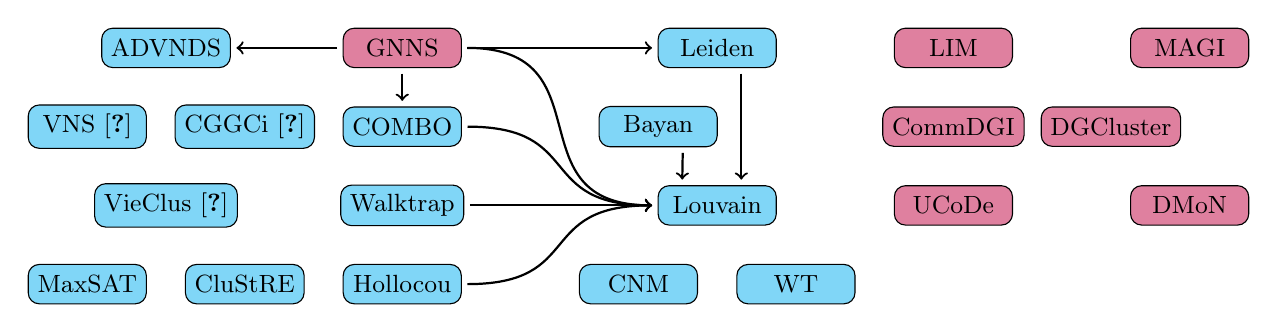
\begin{tikzpicture}[
            paper/.style={
                    draw,
                    rectangle,
                    rounded corners,
                    align=left,
                    font=\small,
                    minimum width=1.5cm,
                    minimum height=0.5cm
                },
            cite/.style={
                    ->,
                    thick,
                    shorten >=2pt,
                    shorten <=2pt
                },
            ae/.style={
                    fill=cyan!50
                },
            ml/.style={
                    fill=purple!50
                },
            node distance=0.3cm
        ]

        \node[paper, ae] (advnds) at (1, 5) {ADVNDS};
        \node[paper, ae] (vns) at (0, 4) {VNS~\cite{vns2012}};
        \node[paper, ae] (cggci) at (2, 4) {CGGCi~\cite{vns2012}};
        \node[paper, ae] (vieclus) at (1, 3) {VieClus~\cite{vieclus2018}};
        \node[paper, ae] (maxsat) at (0, 2) {MaxSAT};
        \node[paper, ae] (clustre) at (2, 2) {CluStRE};
        \node[paper, ml] (gnns) at (4, 5) {GNNS};
        \node[paper, ae] (combo) at (4, 4) {COMBO};
        \node[paper, ae] (walktrap) at (4, 3) {Walktrap};
        \node[paper, ae] (hollocou) at (4, 2) {Hollocou};
        \node[paper, ae] (leiden) at (8, 5) {Leiden};
        \node[paper, ae] (bayan) at (7.25, 4) {Bayan};
        \node[paper, ae] (louvain) at (8, 3) {Louvain};
        \node[paper, ae] (cnm) at (7, 2) {CNM};
        \node[paper, ae] (wt) at (9, 2) {WT};
        \node[paper, ml] (lim) at (11, 5) {LIM};
        \node[paper, ml] (commdgi) at (11, 4) {CommDGI};
        \node[paper, ml] (ucode) at (11, 3) {UCoDe};
        \node[paper, ml] (dgcluster) at (13, 4) {DGCluster};
        \node[paper, ml] (magi) at (14, 5) {MAGI};
        \node[paper, ml] (dmon) at (14, 3) {DMoN};

        \draw[cite] (gnns.east) to[out=0, in=180, looseness=1.5] (louvain.west);
        \draw[cite] (gnns.west) to (advnds.east);
        \draw[cite] (gnns.east) to (leiden.west);
        \draw[cite] (gnns.south) to (combo.north);

        \draw[cite] (combo.east) to[out=0, in=180, looseness=1.5] (louvain.west);

        \draw[cite] (leiden.-40) to (louvain.40);

        \draw[cite] (bayan.-40) to (louvain.150);

        \draw[cite] (walktrap) to (louvain);

        \draw[cite] (hollocou.east) to[out=0, in=180, looseness=1.5] (louvain.west);

        % % ---- Within-column citations ----
        % \draw[cite, bend left=25] (a5.north west) to (a1.south west);
        % \draw[cite, bend left=25] (a5.north west) to (a2.south west);
        % \draw[cite, bend left=25] (a5.north west) to (a3.south west);

        % \draw[cite, bend left=25] (a6.north west) to (a1.south west);
        % \draw[cite, bend left=25] (a6.north west) to (a2.south west);
        % \draw[cite, bend left=25] (a6.north west) to (a3.south west);
        % \draw[cite] (a6) to (a5);

        % \draw[cite, bend right=25] (a7.north east) to (a4.south east);

        % \draw[cite, bend right=25] (a8.north east) to (a2.south east);

        % \draw[cite, bend left=15] (a9.north west) to (a3.south west);

        % \draw[cite] (a10) to (a9);
        % \draw[cite, bend left=10] (a10.north west) to (a1.south west);
        % \draw[cite, bend left=10] (a10.north west) to (a2.south west);
        % \draw[cite, bend left=10] (a10.north west) to (a3.south west);
        % \draw[cite, bend left=10] (a10.north west) to (a3.south west);

        % \draw[cite, bend left=10] (a11.north west) to (a3.south west);
        % \draw[cite, bend left=10] (a11.north west) to (a6.south west);
        % \draw[cite, bend left=10] (a11.north west) to (a7.south west);


        % \draw[cite, bend right=25] (b5.north east) to (b2.south east);
        % \draw[cite, bend right=25] (b5.north east) to (b3.south east);

        % \draw[cite, bend right=25] (b6.north east) to (b3.south east);

        % \draw[cite, bend right=25] (b7.north east) to (b2.south east);
        % \draw[cite, bend right=25] (b7.north east) to (b3.south east);
        % \draw[cite] (b7) to (b6);

        % \draw[cite, bend right=25] (b8.north east) to (b3.south east);

        % \draw[cite, bend right=25] (b9.north east) to (b2.south east);
        % \draw[cite, bend right=25] (b9.north east) to (b6.south east);
        % \draw[cite, bend right=25] (b9.north east) to (b7.south east);

        % % ---- Cross-column citation (intentionally rare) ----
        % \draw[cite, bend right=5] (b4.north west) to (a3.south east);
        % \draw[cite, bend right=5] (b4.north west) to (a9.south east);

        % \draw[cite, bend right=5] (b5.north west) to (a3.south east);

        % \draw[cite, bend right=5] (b8.north west) to (a2.south east);

        % \draw[cite, bend right=5] (b9.north west) to (a3.south east);

        % % ---- Optional: shaded column backgrounds ----
        % \node[fit=(a1)(a4), fill=blue!5, rounded corners, inner sep=6pt] {};
        % \node[fit=(b1)(b4), fill=red!5,  rounded corners, inner sep=6pt] {};

    \end{tikzpicture}

    % Normal caption
    \caption{Experimental comparisons visualized.}
    % Description for someone who can't see (only clear text)
    \Description{Test.}
    \label{fig:comparisons}
\end{figure*}

\ifSubfilesClassLoaded{%
    \bibliography{../paper.bib}%
}{}

\end{document}